\section{Experiments: Model Pipeline}
\label{sec:experiments}

\subsection{Model Pipeline}
\label{subsec:pipeline}

\begin{frame}
    \frametitle{Pipeline for Model Training}
    \begin{figure}
        \centering
        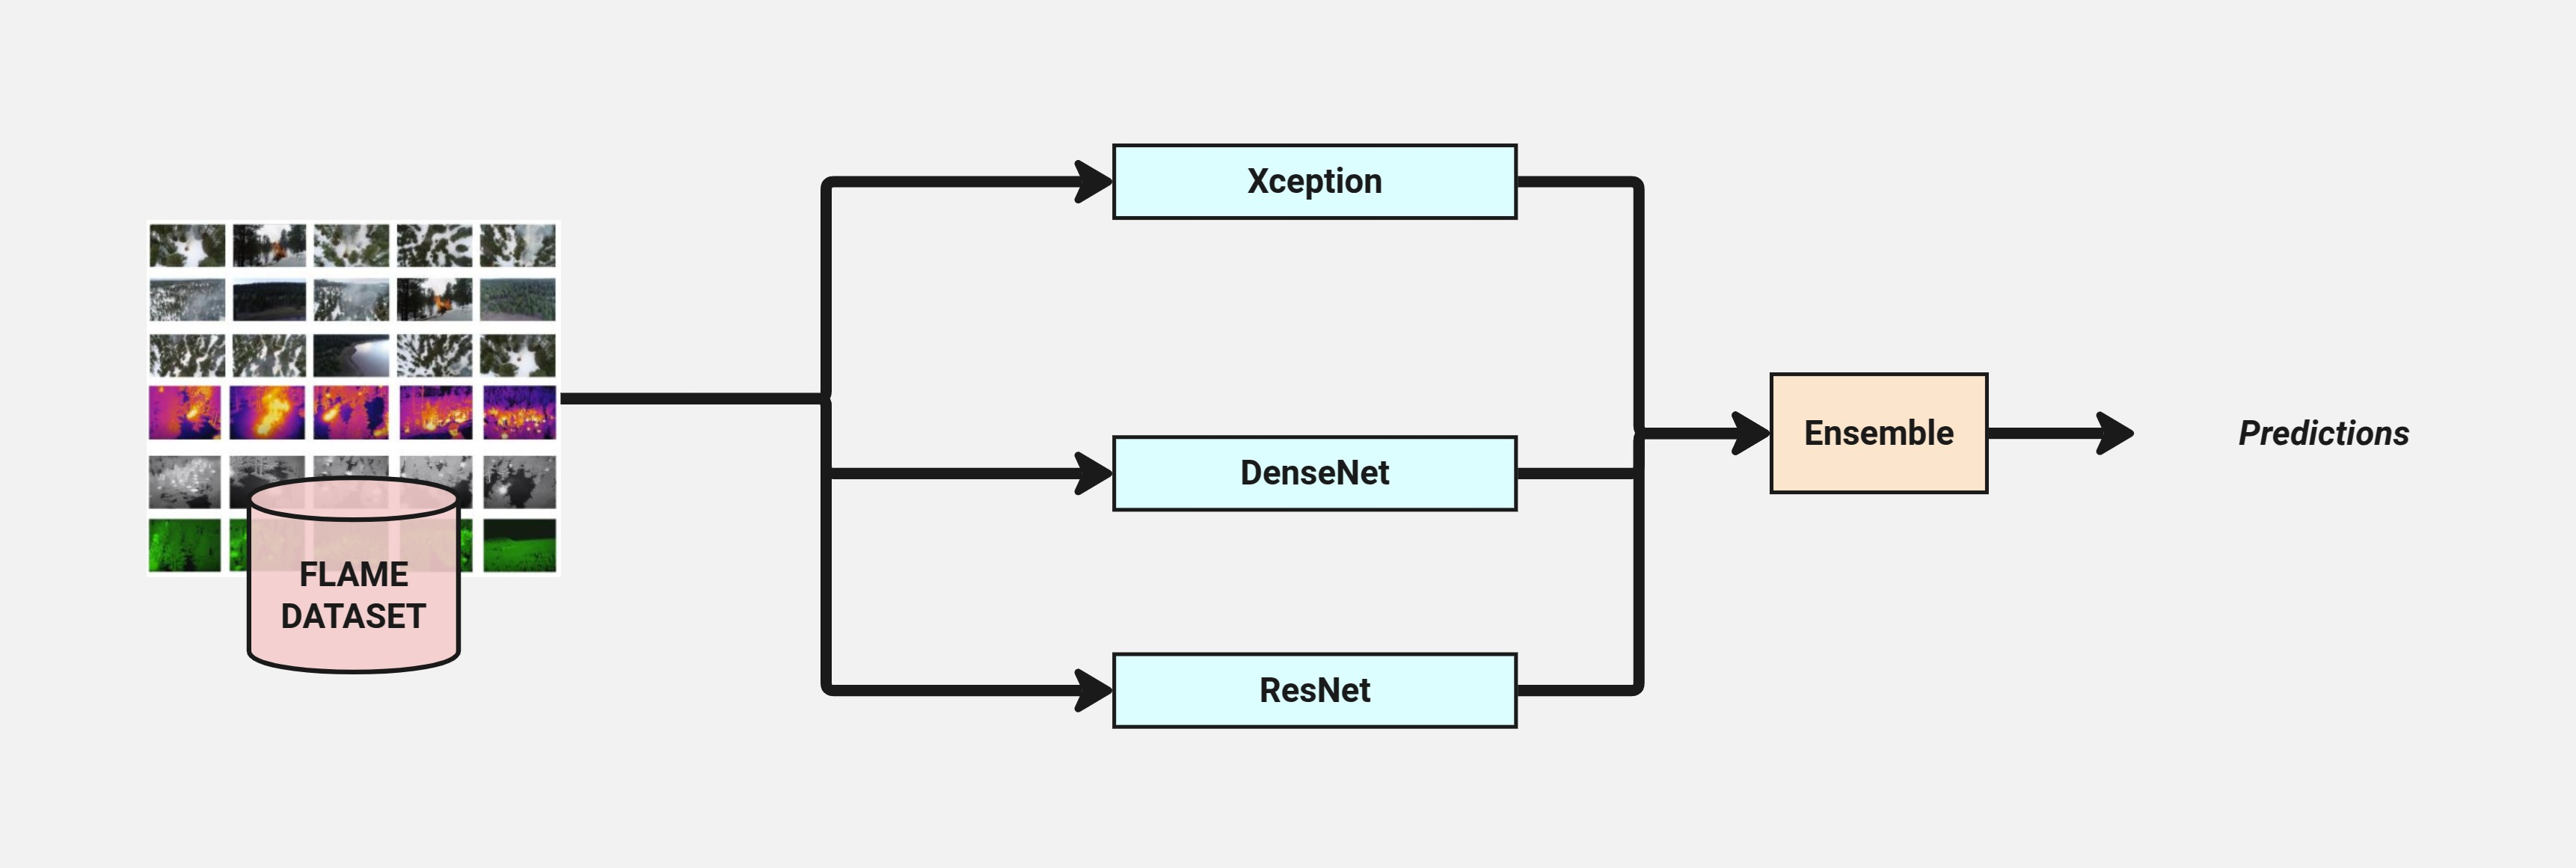
\includegraphics[width=0.7\textwidth]{images/model}
        \caption{Model Architecture}\label{fig:model}
    \end{figure}
    \begin{itemize}
        \item \textbf{Preprocessing:} Images resized to \textbf{224x224} and augmented.
        \item \textbf{Training Strategy:} Individual CNNs trained separately.
        \item \textbf{Evaluation:} Models compared based on \textbf{accuracy}, precision, recall, and \textbf{F1-score}.
    \end{itemize}
\end{frame}

\subsection{Hyperparameter Tuning}
\label{subsec:hyper-tuning}

\begin{frame}
    \frametitle{Keras Tuner for Hyperparameter Search}
    \begin{itemize}
        \item \textbf{Keras Tuner} used for optimizing \textbf{unfrozen layers, dropout, L2 regularization, and learning rate}.
        \item Best hyperparameters found:
    \end{itemize}
    \begin{table}[]
        \centering
        \begin{tabular}{|c|c|c|c|c|}
            \hline
            \textbf{Model} & \textbf{U. layers} & \textbf{Dropout} & \textbf{L2 Factor} & \textbf{L. Rate} \\
            \hline
            Xception & 25 & 0.45 & 0.001 & 0.00541 \\
            DenseNet121 & 20 & 0.35 & 0.001 & 0.00147 \\
            ResNet152 & 45 & 0.4 & 0.0005 & 0.00093 \\
            \hline
        \end{tabular}
    \end{table}
\end{frame}

\subsection{Ensemble}
\label{subsec:ensemble}

\begin{frame}
    \frametitle{Why Use an Ensemble?}
    \begin{itemize}
        \item \textbf{Goal:} Improve model \textbf{stability and accuracy}.
        \item We experimented with:
            \begin{itemize}
                \item Majority Voting (Final Selection).
                \item Weighted Averaging.
                \item Stacking.
            \end{itemize}
    \end{itemize}
    \blocky{Final Approach: Voting}{
        \begin{itemize}
            \item Each model votes on the predicted class.
            \item The most frequent class is the \textbf{final prediction}.
        \end{itemize}
    }
\end{frame}



